\documentclass[xcolor=dvipsnames]{beamer}
\usepackage{graphicx}
\usepackage{xcolor}
\usepackage{tikz}
\usepackage{tikzscale}
\usetikzlibrary{positioning}
\usetikzlibrary{arrows.meta}
\usetikzlibrary{fit}
\usepackage{filecontents}
\usepackage{multicol}
\usepackage[export]{adjustbox}
\usepackage{tcolorbox}
\usepackage{fontspec}
\setsansfont[
ItalicFont=Roboto-LightItalic.ttf
]{Roboto Light}
\graphicspath{{fig/}}

% generalized mean line
\begin{filecontents*}{genmean.tikz}
    \centering
    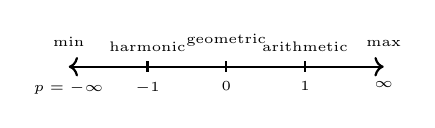
\begin{tikzpicture}
        \tiny
        \draw[thick,<->] (0,0) -- (4,0);
        \foreach \x in {1,2,3} \draw[thick] (\x cm,2pt) -- (\x cm,-2pt);
        \draw (0,0) node[below=3pt] {$ p=-\infty $} node[above=5pt] {min};
        \draw (1,0) node[below=3pt] {$ -1 $} node[above=3pt] {harmonic};
        \draw (2,0) node[below=3pt] {$ 0 $} node[above=5pt] {geometric};
        \draw (3,0) node[below=3pt] {$ 1 $} node[above=3pt] {arithmetic};
        \draw (4,0) node[below=3pt] {$ \infty $} node[above=5pt] {max};
    \end{tikzpicture}
\end{filecontents*}

% define themes
\usecolortheme{dolphin}

% change text to offblack
\definecolor{almostblack}{HTML}{262626}
\setbeamercolor{normal text}{fg=almostblack}

\definecolor{pyred}{HTML}{DA2623}
\definecolor{pyblue}{HTML}{2E7EBC}

% macros
\newcommand{\trento}{T\raisebox{-0.3ex}{R}ENTo}

\definecolor{theme}{RGB}{90,122,163}
\usecolortheme[named=theme]{structure}

\makeatletter
\setbeamertemplate{frametitle}{
  \ifbeamercolorempty[bg]{frametitle}{}{\nointerlineskip}%
  \@tempdima=\textwidth%
  \advance\@tempdima by\beamer@leftmargin%
  \advance\@tempdima by\beamer@rightmargin%
  \begin{beamercolorbox}[sep=0.3cm,left,wd=\the\@tempdima]{frametitle}
    \vbox{}\vskip-2ex%
    \if@tempswa\else\csname beamer@fteleft\endcsname\fi%
    \strut\insertframetitle\strut\par%
    {%
      \ifx\insertframesubtitle\@empty%
      \else%
      {\usebeamerfont{framesubtitle}\usebeamercolor[fg]{framesubtitle}\insertframesubtitle\strut\par}%
      \fi
    }%
    \vskip.45ex%
    \hrule %height .6pt%
    \vskip-1.45ex%
    \if@tempswa\else\vskip-.3cm\fi%
  \end{beamercolorbox}%
}
\makeatother

% clean up footer
\beamertemplatenavigationsymbolsempty
\setbeamertemplate{footline}[frame number]

%inner theme
\useinnertheme{rectangles}
\setbeamertemplate{itemize item}{\raise.30ex\hbox{\vrule width .80ex height .80ex}}
\setbeamertemplate{itemize subitem}{\raise.35ex\hbox{\vrule width .70ex height .70ex}}

%\title{Determining QGP initial conditions and medium properties via Bayesian model-to-data analysis}
\author{J.S. Moreland, J.E. Bernhard, S.A. Bass}
\date{\today}


\begin{document}

\section{Title}

\usebackgroundtemplate{%
\tikz[overlay,remember picture] \node[opacity=0.4, at=(current page.center)] {
   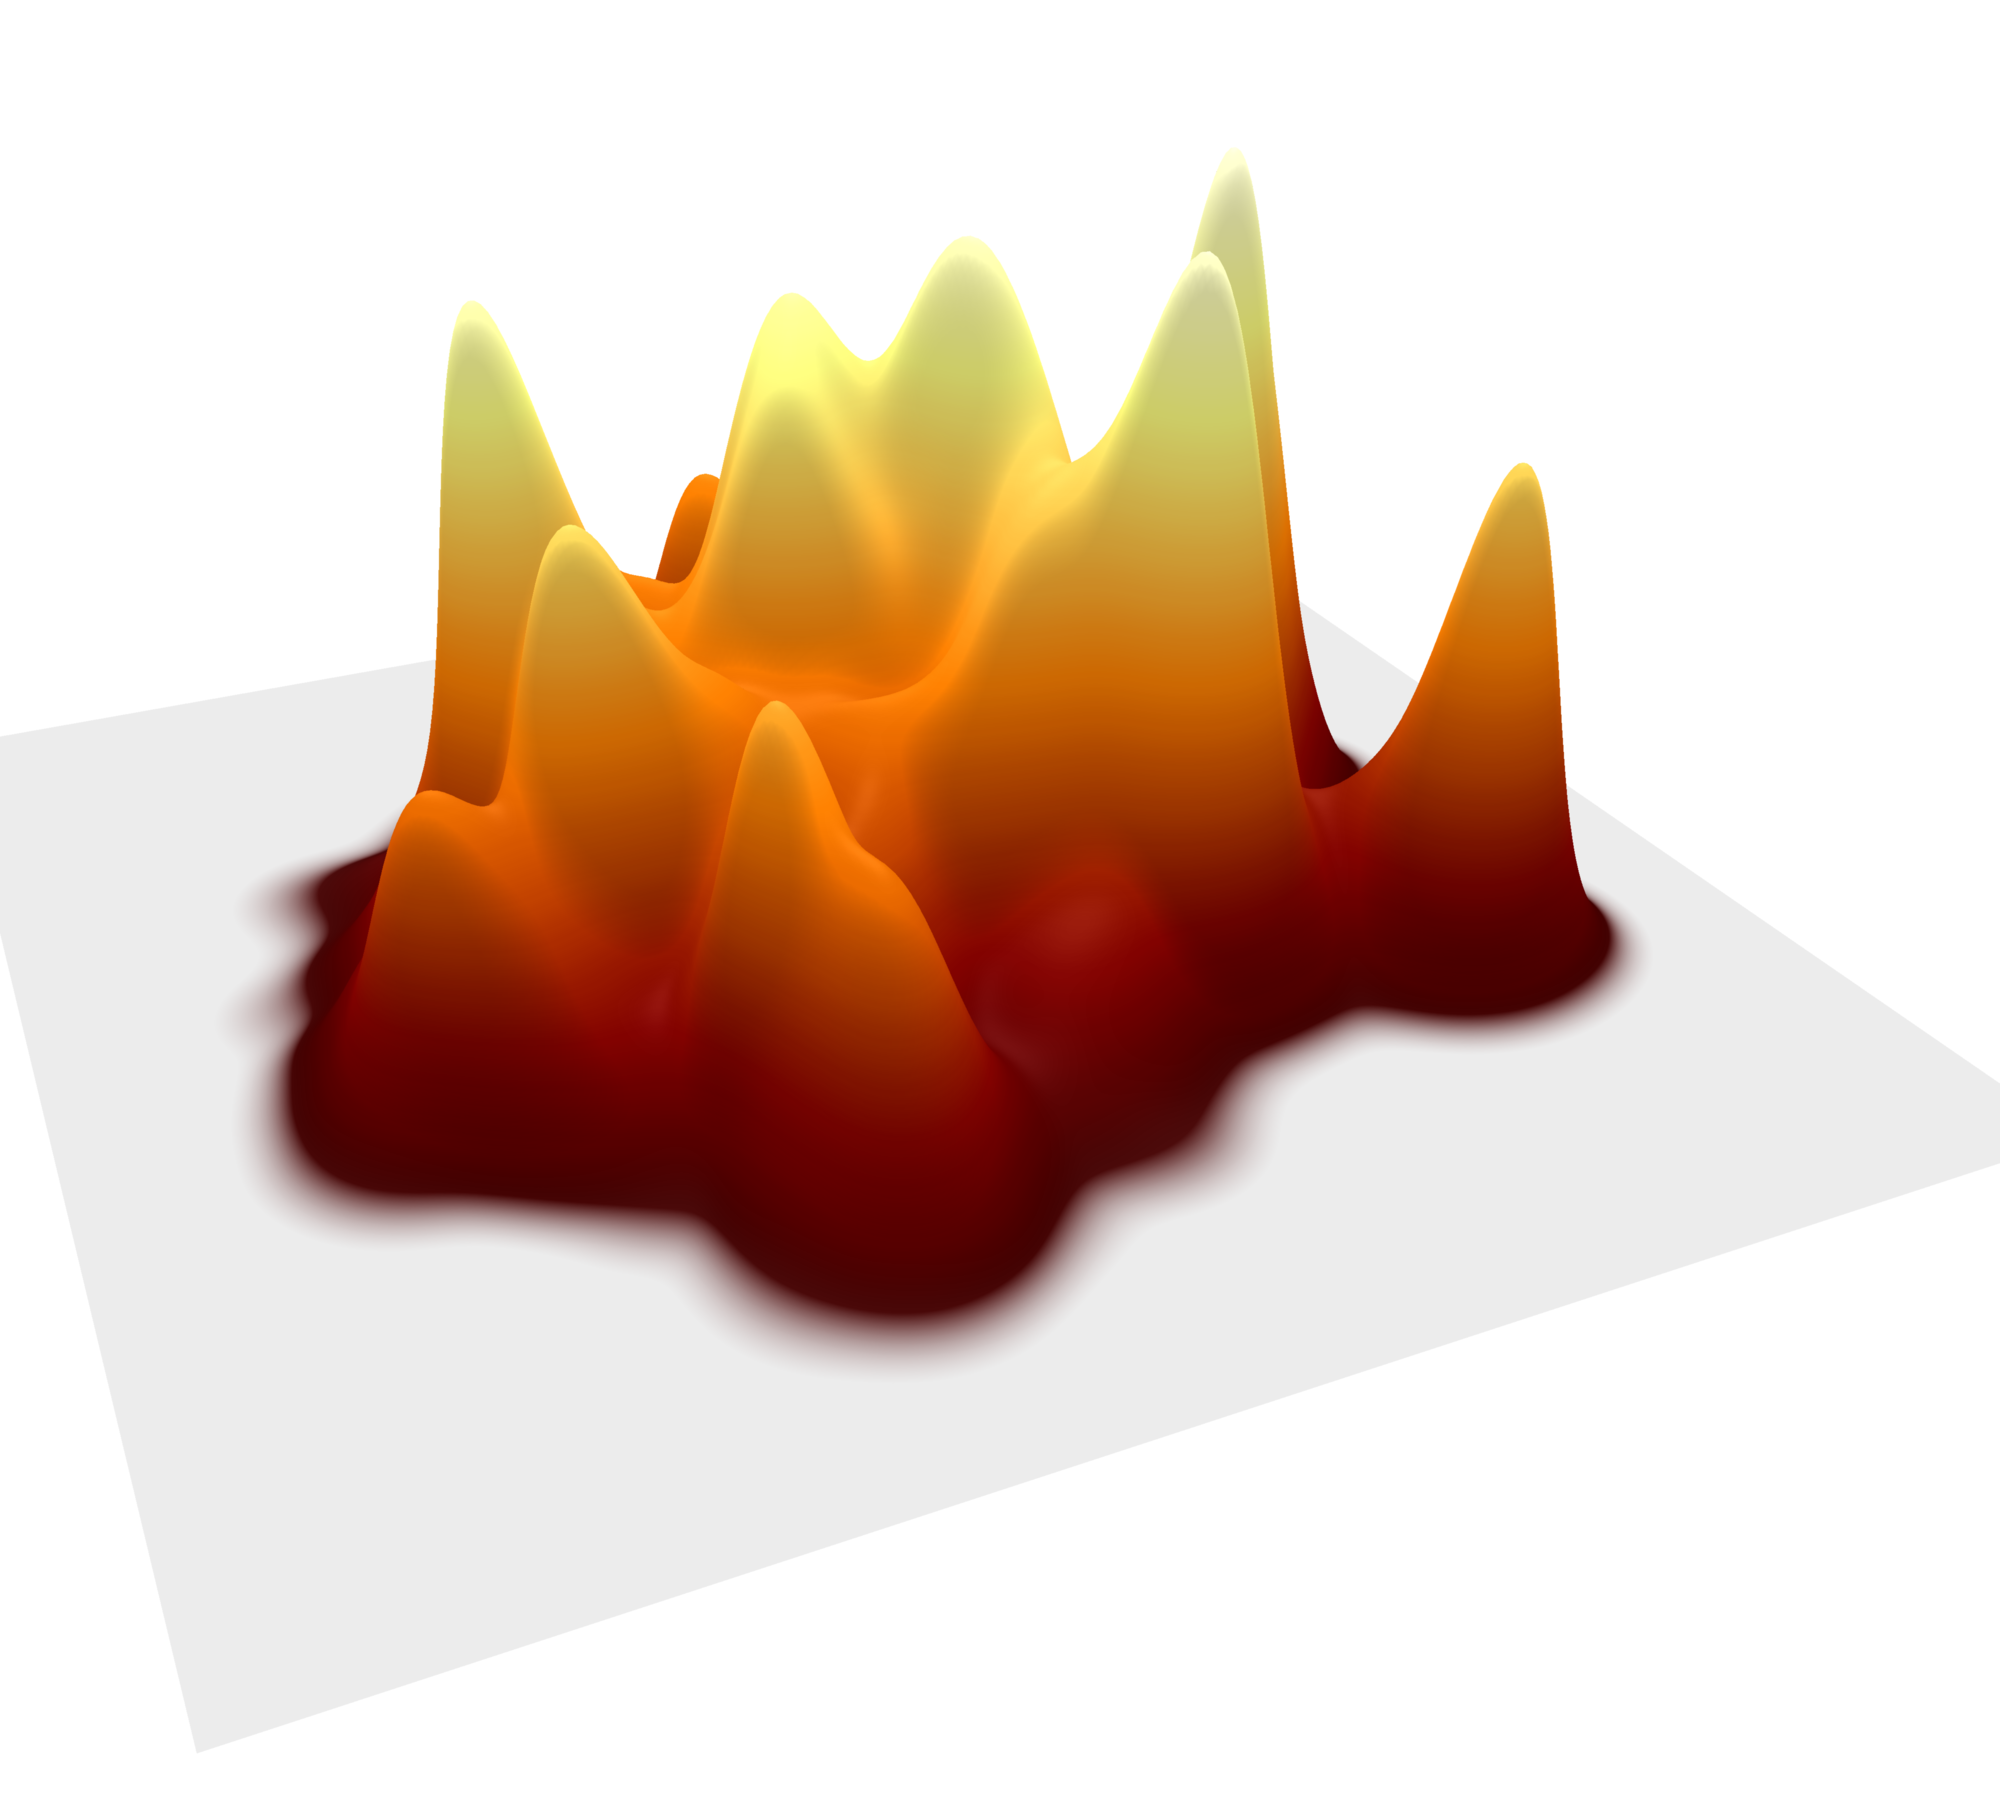
\includegraphics[width=\paperwidth]{trento2}};
}

\frame[plain,noframenumbering]{
  \begin{tikzpicture}[remember picture,overlay]
    \coordinate (middle) at (current page.center);
    \def\sep{.028\paperwidth}
    \def\extra{.6em}
    \node[rectangle, fill=theme, align=center, anchor=center, yshift=2.75cm, fill opacity=0.08, text opacity=1] at (middle) {
      \color{theme} \Large
      Determining QGP initial conditions and medium\\
      \color{theme} \Large
      properties via Bayesian model-to-data analysis
    };
    \node[align=center, anchor=center, yshift=1. cm] at (middle) {
      \insertauthor \\[\extra]
      Initial Stages~$\vert$~\insertdate
    };
    \node[align=center, anchor=center, yshift=-3 cm] at (middle) {
      
\includegraphics[height=1.2cm]{qcdlogo} \hspace{0.2 cm} \hspace{0.2 cm}
      
\includegraphics[height=1.cm]{ssgf} \vspace{0.2 cm} \\
      \tiny Funding provided by DOE Stewardship Science Graduate Fellowship
    };
  \end{tikzpicture}
}

\usebackgroundtemplate{}

\begin{frame}{Why study the QGP initial conditions?}
    \bigskip
    QGP initial state and its various roles {\scriptsize [Angerami IS15' Napa]}: \\
    \begin{itemize}
        \item Initial conditions are interesting in their own right... \\
        \medskip
        One ultimately seeks first principles description of initial entropy 
        deposition and thermalization. \\
        \medskip
        \item Initial conditions are a "nuissance parameter" in hydrodynamic 
              simulations. Needed to extract transport properties, e.g.\ 
              ~$\eta/s$, ~$\zeta/s$, ~$\hat{e}$, ~$\hat{q}$, etc.     
    \end{itemize}
    \medskip
    Deriving QGP IC from first principles is \emph{challenging}...\\ 
    \medskip
    \begin{tcolorbox}[width=\textwidth, colback=theme!10, colframe=theme!0]
        Can we determine the IC from experiment without detailed knowledge of 
        the initial stages of the collision?
        \medskip \centering \\
        What can we learn with such knowledge?
    \end{tcolorbox}
\end{frame}

\begin{frame}{Deconstructing initial condition models}
    \bigskip
    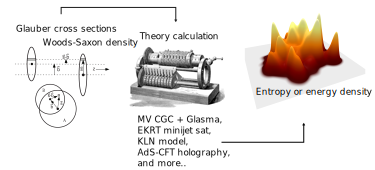
\includegraphics{deconstructing} \\
    \begin{itemize}
        \small
        \item Woods-Saxon, Glauber modeling aspects generally well accepted \\
        \item Useful to separate cross sections and entropy deposition map, \\
        \medskip i.e.\ ~~$dS/dy \sim f(\tilde{T}_A, \tilde{T}_B)$ where $\tilde{T}$ 
                 is a participant thickness or \\
        \smallskip wounded nucleon density. \emph{The mapping $f$ is some 2D surface.}
    \end{itemize}
\end{frame}

\begin{frame}{Parametrizing the initial conditions}
    \vfill
    \begin{columns}
        \begin{column}{0.45\textwidth}
            \vfill
            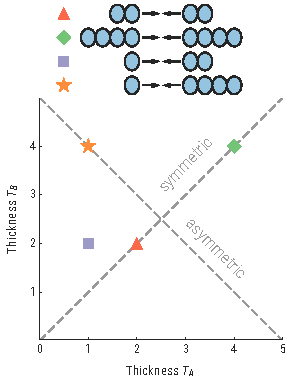
\includegraphics{mapping}
        \end{column}
        \vline
        \begin{column}{0.55\textwidth}
            \smallskip
            \centering \small Generalized mean ansatz: \\
            \smallskip {\large $\frac{dS}{d^2r dy} \propto \Bigl(\frac{T_A^p + T_B^p}{2}\Bigr)^{1/p} $} \\
            \medskip
            \includegraphics{genmean.tikz} \\
            \bigskip \smallskip
            \includegraphics{thickness} 
        \end{column}
    \end{columns}
\end{frame}

\begin{frame}{Reproducing existing IC models}
    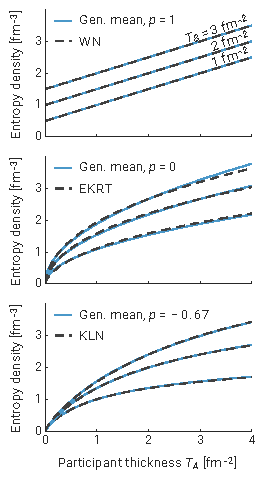
\includegraphics{cgc_compare} \\
    \begin{itemize}
        \item KLN model: \quad $dS/dy \sim Q^2_{s,\text{min}} \Big[2 + \log \Big(\frac{Q^2_{s,\text{max}}}{Q^2_{s,\text{min}}}\Big) \Big]$
        \item EKRT model: \quad $dS/dy \sim$
        \item WN model: \quad $dS/dy \propto T_A + T_B$
    \end{itemize}
\end{frame}

\begin{frame}{\trento\ initial condition model \quad{\scriptsize Phys.\ Rev.\ C {\bf 92}, no.\ 1, 011901 (2015)}}
    \vspace{.6 cm}
    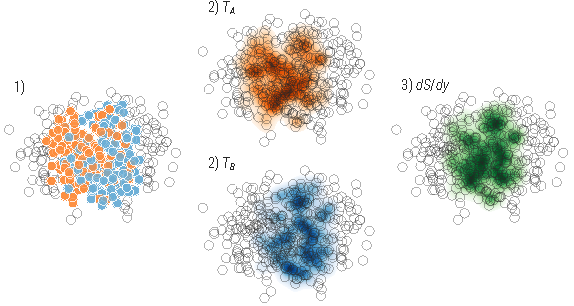
\includegraphics{schematic} \\
    \begin{enumerate}
        \scriptsize
        \setbeamercolor{item projected}{bg=theme!40, fg=almostblack}
        \item Calc participants: $P_\text{coll}(b) = 1 - \exp[-\sigma_{gg} T_{pp}(b)]$, \quad $\int 2 \pi\, b\, db\, P_\text{coll}(b) = \sigma_\text{NN}^\text{inel}$ \\ \vspace{0.1 cm}
        \item Build participant density: $T_A(x,y) = \sum\limits_{i=1}^{N_{\text{part},A}} \gamma_i T_p(x-x_i, y-y_i)$, \quad $\gamma \sim \Gamma(k, 1/k)$ \\
        \item Parameterize entropy deposition w/ generalized mean: $dS/dy \propto \bigg(\frac{T_A^p + T_B^p}{2} \bigg)^{1/p}$
    \end{enumerate}
\end{frame}

\usebackgroundtemplate{%
\tikz[overlay,remember picture] \node[at=(current page.center)] {
   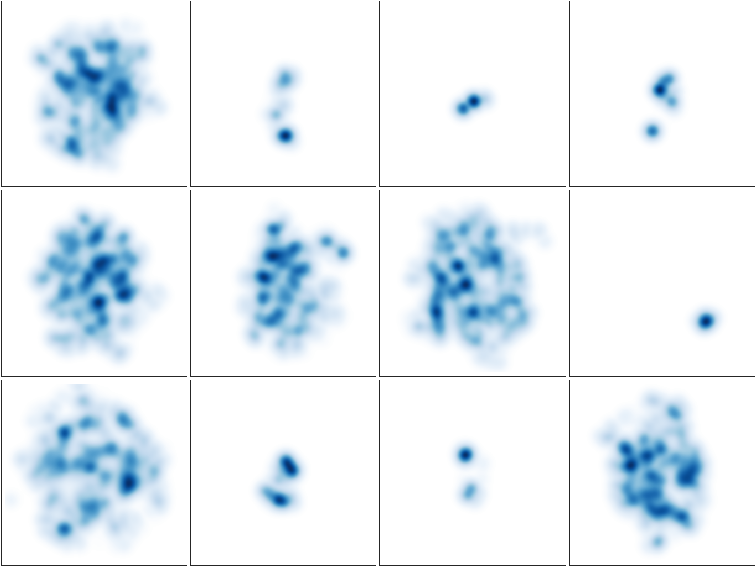
\includegraphics[width=\paperwidth]{trento_minbias}};
}

\begin{frame}
\end{frame}

\usebackgroundtemplate{}

\begin{frame}{Modern event-by-event hybrid model}
    \bigskip
    \begin{itemize}
        \item \trento\ initial conditions \\
        {\scriptsize Moreland, Bernhard, Bass, PRC {\bf 92}, no.\ 1, 011901 (2015)} \\
        \begin{table}
            \scriptsize \flushleft
            \begin{tabular}{r l}
                norm & entropy normalization \\ 
                $p$ & entropy deposition parameter \\
                $k$ & proton-proton multiplicity fluctuations \\
                $w$ & Gaussian nucleon width
            \end{tabular}
        \end{table}
        \medskip
        \item HotQCD equation of state \\
        {\scriptsize Bazavov, et.\ al.\ PRD {\bf 90}, 094503 (2014)} \\
        \smallskip 
        \item iEBE-VISHNU hydrodynamics \\
        {\scriptsize Shen, Qiu, Song, Bernhard, Bass, Heinz, Comp.\ Phys.\ Comm.\ {\bf 199}, 61 (2016)}  
        \begin{table}
            \scriptsize \flushleft
            \begin{tabular}{r l}
                $\eta/s$ min & shear viscosity minimum \\ 
                $\eta/s$ slope & shear viscosity slope \\
                $\zeta/s$ norm & bulk viscosity normalization \\
                $T_\text{sw}$ & hydro-to-urqmd switching temp
            \end{tabular}
        \end{table}
        \medskip
        \item UrQMD hadronic afterburner \\
        {\scriptsize Bass et.\ al, Prog.\ Part.\ Nucl.\ Phys.\ {\bf 41}, 255 (1998)} \\
        {\scriptsize Bleicher et.\ al, J.\ Phys.\ G {\bf 25}, 1859 (1999)}
    \end{itemize}
\end{frame}

\begin{frame}{The challenge of rigorous model-to-data comparison}
   
    \begin{tikzpicture}[overlay, remember picture]
        \node [anchor=east, left=1cm of current page.north, yshift=-1.6cm] (t1) {\large Parameter};
        \node [anchor=west, right=1cm of current page.north, yshift=-1.6cm] (t2) {\large Observable};
        
        \node [anchor=east, left=1cm of current page.north, yshift=-2.2cm] (a1) {\small shear viscosity};
        \node [anchor=east, left=1cm of current page.north, yshift=-2.7cm] (a2) {\small bulk viscosity};
        \node [anchor=east, left=1cm of current page.north, yshift=-3.2cm] (a3) {\small pre-equilibrium flow};
        \node [anchor=east, left=1cm of current page.north, yshift=-3.7cm] (a4) {\small nucleon width};
        \node [anchor=east, left=1cm of current page.north, yshift=-4.2cm] (a5) {\small hadronization temp};
        \node [anchor=east, left=1cm of current page.north, yshift=-4.7cm] (a6) {\small p+p fluctuations};

        \node [anchor=west, right=1cm of current page.north, yshift=-2.2cm] (b1) {\small identified yields};
        \node [anchor=west, right=1cm of current page.north, yshift=-2.7cm] (b2) {\small identified mean $p_T$};
        \node [anchor=west, right=1cm of current page.north, yshift=-3.2cm] (b3) {\small flow cumulants};
        \node [anchor=west, right=1cm of current page.north, yshift=-3.7cm] (b4) {\small mode mixing observables};
        \node [anchor=west, right=1cm of current page.north, yshift=-4.2cm] (b5) {\small event plane decorrelations};
        \node [anchor=west, right=1cm of current page.north, yshift=-4.7cm] (b6) {\small HBT interferometry};

        \draw [almostblack, line width=0.2pt] (a1.east) -- (b1.west);
        \draw [almostblack, line width=0.2pt] (a1.east) -- (b2.west);
        \draw [almostblack, line width=0.2pt] (a1.east) -- (b3.west);
        \draw [almostblack, line width=0.2pt] (a1.east) -- (b4.west);
        \draw [almostblack, line width=0.2pt] (a1.east) -- (b5.west);
        \draw [almostblack, line width=0.2pt] (a1.east) -- (b6.west);
        
        \draw [almostblack, line width=0.2pt] (a2.east) -- (b1.west);
        \draw [almostblack, line width=0.2pt] (a2.east) -- (b2.west);
        \draw [almostblack, line width=0.2pt] (a2.east) -- (b3.west);
        \draw [almostblack, line width=0.2pt] (a2.east) -- (b4.west);
        \draw [almostblack, line width=0.2pt] (a2.east) -- (b5.west);
        \draw [almostblack, line width=0.2pt] (a2.east) -- (b6.west);
        
        \draw [almostblack, line width=0.2pt] (a3.east) -- (b1.west);
        \draw [almostblack, line width=0.2pt] (a3.east) -- (b2.west);
        \draw [almostblack, line width=0.2pt] (a3.east) -- (b3.west);
        \draw [almostblack, line width=0.2pt] (a3.east) -- (b4.west);
        \draw [almostblack, line width=0.2pt] (a3.east) -- (b5.west);
        \draw [almostblack, line width=0.2pt] (a3.east) -- (b6.west);

        \draw [almostblack, line width=0.2pt] (a4.east) -- (b1.west);
        \draw [almostblack, line width=0.2pt] (a4.east) -- (b2.west);
        \draw [almostblack, line width=0.2pt] (a4.east) -- (b3.west);
        \draw [almostblack, line width=0.2pt] (a4.east) -- (b4.west);
        \draw [almostblack, line width=0.2pt] (a4.east) -- (b5.west);
        \draw [almostblack, line width=0.2pt] (a4.east) -- (b6.west);

        \draw [almostblack, line width=0.2pt] (a5.east) -- (b1.west);
        \draw [almostblack, line width=0.2pt] (a5.east) -- (b2.west);
        \draw [almostblack, line width=0.2pt] (a5.east) -- (b3.west);
        \draw [almostblack, line width=0.2pt] (a5.east) -- (b4.west);
        \draw [almostblack, line width=0.2pt] (a5.east) -- (b5.west);
        \draw [almostblack, line width=0.2pt] (a5.east) -- (b6.west);
        
        \draw [almostblack, line width=0.2pt] (a6.east) -- (b1.west);
        \draw [almostblack, line width=0.2pt] (a6.east) -- (b2.west);
        \draw [almostblack, line width=0.2pt] (a6.east) -- (b3.west);
        \draw [almostblack, line width=0.2pt] (a6.east) -- (b4.west);
        \draw [almostblack, line width=0.2pt] (a6.east) -- (b5.west);
        \draw [almostblack, line width=0.2pt] (a6.east) -- (b6.west);
    \end{tikzpicture}
    \vspace{3.5 cm} \\
    \begin{tcolorbox}[width=\textwidth, colback=theme!10, colframe=theme!0]
        \centering
        \small Testing a single set of parameters requires $\mathcal{O}(10^4)$ hydro events \\
        \small \smallskip ...and evaluating eight different parameters five times each\\ requires $5^8 \times 10^4 \approx 10^9$ hydro events. \bigskip \\
        {\large That's roughly $10^5$ computer \emph{years}!}
    \end{tcolorbox}
\end{frame}

\begin{frame}{Solution: modern Bayesian methodology}
    \begin{columns}
        \begin{column}{0.5\textwidth}
            \begin{enumerate}
                \item Replace factorial design with Latin hypercube
            \end{enumerate}
        \end{column}
        \vline
        \begin{column}{0.5\textwidth}
        \end{column}
    \end{columns}
\end{frame}

\begin{frame}{Calibrating the model: before and after}
    \medskip
    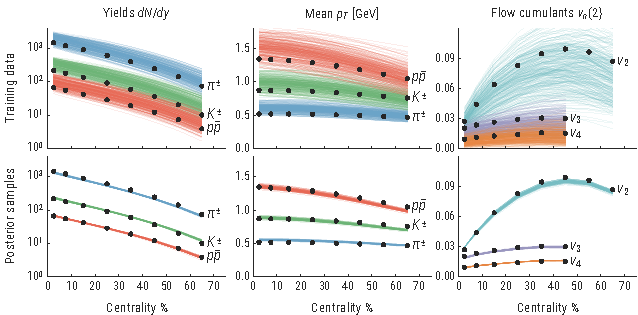
\includegraphics{observables_plot} \\
    \bigskip
    \begin{itemize}
        \small
        \item Top: run model ($\times 10^4$ events) at each design point ($\times300$ evals)
        \vspace{0.2 cm}
        \item Bottom: emulator predictions for 100 samples from the posterior
    \end{itemize}
\end{frame}

\begin{frame}{Running the model with high probability parameters}
    \vfill
    \centering
    \begin{columns}
        \begin{column}{0.4\textwidth}
            \scriptsize
            \begin{itemize}
                \item Choose high probability model param.\ from Bayesian posterior (listed right)
                \smallskip
                \item Run full hybrid model using high probability parameters (shown bottom)
            \end{itemize}
        \end{column}
        \begin{column}{0.6\textwidth}
            \scriptsize
            \begin{tabular}{lllll}
                \multicolumn{2}{c}{Initial condition} & & \multicolumn{2}{c}{QGP medium} \\
                \noalign{\smallskip}\hline\noalign{\medskip}
                norm & 120.          &&  $\eta/s$ min   & 0.08       \\
                $p$  & 0.0           &&  $\eta/s$ slope & 0.85 GeV$^{-1}$   \\
                $k$  & 1.5           &&  $\zeta/s$ norm & 1.25       \\
                $w$  & 0.43 fm       &&  $T_\text{sw}$  & 0.148 GeV  \\
            \end{tabular}
        \end{column}
    \end{columns}
    \vspace{0.5 cm}
    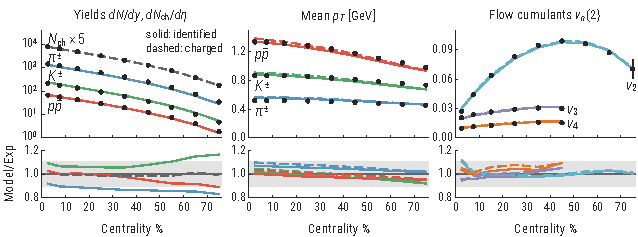
\includegraphics{mode_observables}
\end{frame}

\begin{frame}
    \begin{columns}
        \begin{column}{1 cm}
            \centering
            \hspace{0.5 cm}
            \rotatebox[origin=c]{90}{\scriptsize \only<1>{\color{pyblue}} 
            \only<2->{\color{pyblue!40}} Calibrated to identified particles}
        \end{column}
        \begin{column}{\paperheight}
            \centering \vspace{0.3 cm}\\
            \begin{tikzpicture}
                \only<1>{\node [opacity=1] (post) {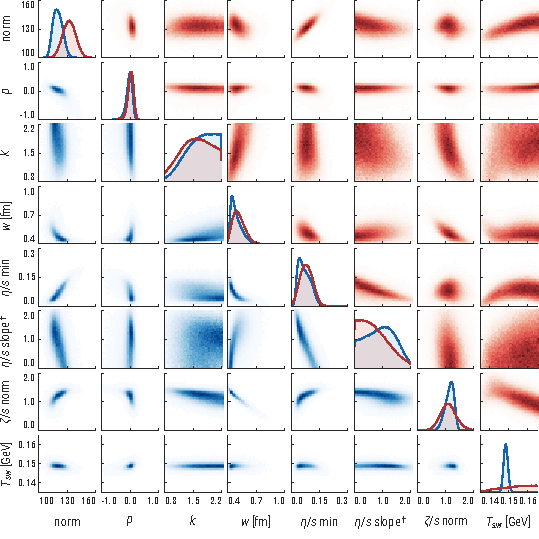
\includegraphics{posterior}};}
                \only<2->{\node [opacity=0.3] (post) {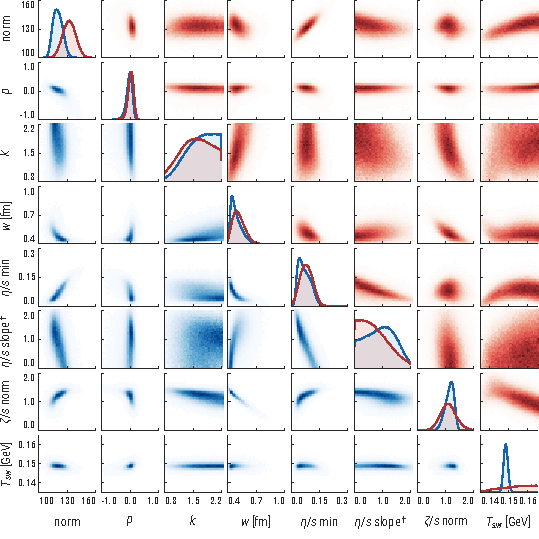
\includegraphics{posterior}};}
            \end{tikzpicture}
        \end{column}
        \begin{column}{1 cm}
            \centering
            \rotatebox[origin=c]{-90}{\scriptsize \only<1>{\color{pyred}} 
            \only<2->{\color{pyred!40}} Calibrated to charged particles}
            \hspace{0.4 cm}
        \end{column}
    \end{columns}

    \only<2>{
    \begin{tikzpicture}[remember picture, overlay]
        \filldraw [draw=almostblack, fill=almostblack, overlay, opacity=0.1, anchor=center] (current page.south west) rectangle (\pagewidth,\pagewidth);
        \node[inner sep=0pt, yshift=1cm, overlay] (node1) at (current page.center) {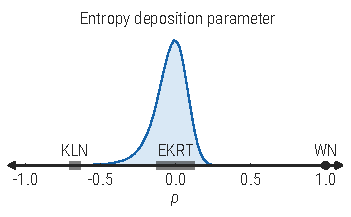
\includegraphics{posterior_p_arrows}};
        \node[inner sep=0pt, below=2ex of node1.south, anchor=north] {
            \begin{tcolorbox}[width=0.552\textwidth, boxrule=0pt, colback=white, colframe=almostblack, sharp corners]
                \scriptsize \centering
                Generalized mean parametrization: \medskip \\
                $dS/dy \propto \Big(\frac{T_A^p + T_B^p}{2}\Big)^{1/p}$
            \end{tcolorbox}
        };
    \end{tikzpicture}}

    \only<3>{
    \begin{tikzpicture}[remember picture, overlay]
        \filldraw [draw=almostblack, fill=almostblack, overlay, opacity=0.1, anchor=center] (current page.south west) rectangle (\pagewidth,\pagewidth);
        \node[inner sep=0pt, yshift=1cm, overlay] at (current page.center) {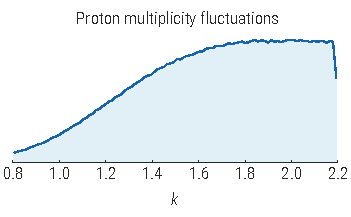
\includegraphics{posterior_k}};
        \node[inner sep=0pt, below=2ex of node1.south, anchor=north] {
            \begin{tcolorbox}[width=0.552\textwidth, boxrule=0pt, colback=white, colframe=almostblack, sharp corners]
                \scriptsize \centering
                Random Gamma nucleon weights: \medskip \\
                $P(\gamma\, \vert\, k) = \frac{k^k}{\Gamma(k)} \gamma^{k - 1} e^{-k \gamma}$ \\ 
                $T_A(x,y) = \sum\limits_{i=1}^{N_{\text{part},A}} \gamma_i T_p(x-x_i, y-y_i)$
            \end{tcolorbox}
        };
    \end{tikzpicture}}

    \only<4>{
    \begin{tikzpicture}[remember picture, overlay]
        \filldraw [draw=almostblack, fill=almostblack, overlay, opacity=0.1, anchor=center] (current page.south west) rectangle (\pagewidth,\pagewidth);
        \node[inner sep=0pt, yshift=1cm, overlay] at (current page.center) {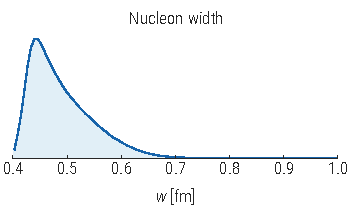
\includegraphics{posterior_w}};
        \node[inner sep=0pt, below=2ex of node1.south, anchor=north] {
            \begin{tcolorbox}[width=0.552\textwidth, boxrule=0pt, colback=white, colframe=almostblack, sharp corners]
                \scriptsize \centering
                Gaussian nucleon thickness: \medskip \\
                $T_p(x,y) = \frac{1}{2 \pi w^2} e^{-(x^2 +y^2)/(2w^2)}$
            \end{tcolorbox}
        };
    \end{tikzpicture}}

    \only<5>{
    \begin{tikzpicture}[remember picture, overlay]
        \filldraw [draw=almostblack, fill=almostblack, overlay, opacity=0.1, anchor=center] (current page.south west) rectangle (\pagewidth,\pagewidth);
        \node[inner sep=0pt, yshift=1cm] at (current page.center) {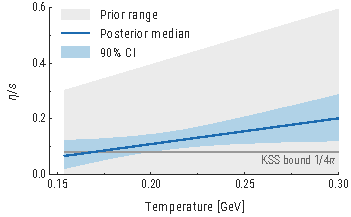
\includegraphics{etas_estimate}};
        \node[inner sep=0pt, below=2ex of node1.south, anchor=north] {
            \begin{tcolorbox}[width=0.552\textwidth, boxrule=0pt, colback=white, colframe=almostblack, sharp corners]
                \scriptsize \centering
                Shear viscosity parametrization: \medskip \\
                $(\eta/s)(T) = (\eta/s)_\text{min} + (T - T_c) (\eta/s)_\text{slope}$ 
            \end{tcolorbox}
        };
    \end{tikzpicture}}
    
\end{frame}

\begin{frame}{Conclusions}
\medskip
Initial condition properties
\begin{itemize}
    \item Yields, mean $p_T$ and flows impose strong constraints on IC. \\
    \item Entropy  deposition mimic'd by $dS/dy \sim \sqrt{T_A T_B}$ \\
    \item Data strongly prefers small nucleon width $w \approx 0.4\mathrm{-}0.5$ fm! \\
    \item A+A collisions weakly sensitive to p+p mult.\ fluctuations \\
    \item Prefered initial conditions similar to EKRT, IP-Glasma \\
\end{itemize}
\smallskip
Hydrodynamic transport properties
\begin{itemize}
    \item First quantitative credibility interval on $(\eta/s)(T)$!
    \item Data prefers non-zero bulk viscosity
    \item Hydro-to-micro $T_\text{sw}$ determined by relative species yields 
\end{itemize}
\vfill
\trento\ is publicly available at \url{qcd.phy.duke.edu/trento}
\end{frame}
\end{document}
